\documentclass[conference]{IEEEtran}
\IEEEoverridecommandlockouts
% The preceding line is only needed to identify funding in the first footnote. If that is unneeded, please comment it out.
%\usepackage{cite}
\usepackage{amsmath,amssymb,amsfonts}
\usepackage{algorithmic}
\usepackage{graphicx}
\usepackage{textcomp}
\usepackage{xcolor}
%\def\BibTeX{{\rm B\kern-.05em{\sc i\kern-.025em b}\kern-.08em
%		T\kern-.1667em\lower.7ex\hbox{E}\kern-.125emX}}

\usepackage{hyperref}
\usepackage{biblatex} 
\addbibresource{refs.bib}

\begin{document}
	
	\title{Characterizing Deprived Urban Areas Using Remote Sensing}

	\author{\IEEEauthorblockN{1\textsuperscript{st} Yvette Espinoza}
		\IEEEauthorblockA{\textit{Software Engineer} \\
			\textit{Northrop Grumman}\\
			Redondo Beach, CA, USA \\
			yespinoz@purdue.edu}
	}

	\maketitle

% ------------------------------------------------------------------------------------------------------------
% ~ ~ ~ ~ ~ ~ ~ ~ ~ ~ ~ ~ ~ ~ ~ ~ ~ ~ ~ ~ ~ ~ ~ ~ ~ ~ ~ ~ ~ ~ ~ ~ ~ ~ ~ ~ ~ ~ ~ ~ ~ ~ ~ ~ ~ ~ ~ ~ ~ ~ ~ ~ ~ ~ 
% ------------------------------------------------------------------------------------------------------------
	\begin{abstract}
		The urban population has increased dramatically in the last few decades, but the rapid rate of urbanization has caused a strain on the available resources, leaving many to live in deprived, or impoverished areas.
		To address these socio-demographic issues policymakers typically rely on traditional survey-based data, like the census, but such data is complex to acquire and can quickly become outdated. Earth observations are the proposed solution to the gaps left by traditional data.
		Artificial intelligence and deep learning algorithms are being used to detect changes on the earth's surface, such as detecting new urban areas.
		New research has focused on classifying elements of the city itself, monitoring waste disposal sites and traffic to have a better understanding of the deprived areas and their needs.
		This project will analyze urban characteristics, what makes an area ‘deprived’, and discuss the uses of remote sensing in socio-demographic applications by collecting and preprocessing SAR data that would be used for classification.

	\end{abstract}

% ------------------------------------------------------------------------------------------------------------
% ~ ~ ~ ~ ~ ~ ~ ~ ~ ~ ~ ~ ~ ~ ~ ~ ~ ~ ~ ~ ~ ~ ~ ~ ~ ~ ~ ~ ~ ~ ~ ~ ~ ~ ~ ~ ~ ~ ~ ~ ~ ~ ~ ~ ~ ~ ~ ~ ~ ~ ~ ~ ~ ~ 
% ------------------------------------------------------------------------------------------------------------
	\section{Literature Review}
		It is estimated that half of the world's population is currently living in cities, with that number expected to rise to 60\% by 2030, but the rapid rate of urbanization has not resulted in an equal increase in public amenities or affordable housing \cite{UN_Sustanability_Report}.
		The lack of affordable housing has led to the creation of informal settlements, commonly referred to as 'slums', or deprived urban areas (DUA).
		These areas of concentrated poverty often lack public amenities such as access to clean water or waste disposal, and are known to have hazardous effects on the inhabitants health \cite{Georgano_Stefanos_2021}.
		
		Poverty reduction, listed in the United Nation's Sustainable Development Goals, is a priority worldwide, though policies enacted and definition of poverty itself vary between countries.
		Some common definitions include the current financial status of residents, or the value of a household's assets, but such methods alone do not paint a clear picture of the situation, since low income households do not necessarily belong to a deprived area \cite{Merodio_Paloma_2021}. 
		Since research has found poverty is related to population growth, one reduction approach focuses on addressing deprived urban areas, thus improving living conditions and reducing the risk of natural hazards \cite{Lin_Li_2021}.
		
		The traditional methods for mapping deprived areas rely on field surveys, such as the census, however these methods are costly and have a long period between collections.
		Since settlements are constantly changing, the data quickly becomes outdated and unable to provide feedback on whether any policies are effective \cite{Williams_Trecia_2020}.
		The COVID-19 pandemic brought more attention to this problem when many field surveys were delayed during a time when data was needed to divert resources to the most affected communities.
		One solution to fill the data gaps left by the traditional methods is to use remote sensing.
		
	\subsection{Remote Sensing}
		There are many ways in which remote sensing can be used to get a better understanding of an area.
		At a high level, satellite images can be used to train deep learning models that classify areas as urban or rural \cite{Guo_Jinxin_2019}, but research has also focused on smaller features, such as waste piles and vehicles.
		
		Radar systems are desirable for data collection because they are not affected by weather conditions such as clouds or lighting.
		The X band of Synthetic Aperture Radars (SAR), which has frequencies in the range of 8-12 GHz, produces high resolution images that can be analyzed for feature extraction \cite{Wurm_2017}.
		The C band, operating from 4-8 GHz, though not as high resolution as the X band, can penetrate deeper, making it a good option for classifying landscapes \cite{Hu_2018}. 
		A disadvantage to SAR is the lack of large datasets that can be used for training the models that extract features from urban areas \cite{Shi_Wenzhong_2020}, but its independence of atmospheric conditions and cloud cover make it a more reliable source of data. 


	\subsection{Polarimetry}
		Dual polarization, where a signal is transmitted in one polarization and received in both polarization's, either HH/HV or VV/VH, is used to provide additional surface details. 
		% YVETTE - maybe have more description here on the polarimetric features, since already have section on texture analysis
		
		
	\subsection{Texture Analysis}
		Texture analysis, characterizing an image by its texture content, is commonly used in remote sensing because of its effectiveness in classification \cite{Huang_2014}.
		One form of texture analysis uses the gray level co-occurrence matrix (GLCM) which contains a mapping of how often a pixel with intensity $i$ appears alongside a pixel of intensity $j$.
		The GLCM can be used to extract 14 texture statistics, with the most commonly used shown in Table \ref{tab:glcm_formulas} where $P_{ij}$ is the $(i,j)$ entry in the matrix. 
		
		% https://rstudio-pubs-static.s3.amazonaws.com/536921_af2c31c083544a3a9588da9c86692636.html
		\begin{table}[htbp]
			\caption{Common GLCM Statistics}
			\centering
			\begin{tabular}{ll} % creating 2 columns left aligned
				\\[1ex]
				Statistic & Formula \\ % Entering row contents
				\hline\hline %inserting double-line
				Energy & $\displaystyle\sum_{i,j=0}^{N-1} P_{ij}^2$ \\
				Contrast & $\displaystyle\sum_{i,j=0}^{N-1} P_{ij}(i-j)^2$ \\
				Entropy & $\displaystyle\sum_{i,j=0}^{N-1} P_{ij}(-ln(P_{ij}))$ \\
				Variance & $\sigma_i = \displaystyle\sum_{i=0}^{N-1} P_{ij}(i-\mu_i)^2$ \\[1ex] % [1ex] adds vertical space
				\hline % inserts single-line
			\end{tabular}
			\label{tab:glcm_formulas}
		\end{table}

		Of the texture statistics, variance has the best performance when differentiating between DUA's and formal areas, since a high variance gives a sharp change in the pixels that usually denote building edges or a drastic change in the environment \cite{Kuffer_2015}.
		The other statistics also provide valuable information, with contrast used to map DUA expansions and entropy as a validation step, since DUA's naturally have high entropy \cite{Kuffer_2016}.
		
	\subsection{Individual Contribution}
		% Access Sentinel-1 data (list specifics), use the SNAP program to preprocess the data that will be used to classify the 17 local climate zones listed in the Hu_2018 paper.  
		For the individual contribution the data collection and processing from \cite{Hu_2018} will be implemented. 
		Sentinel-1 dual-pol SAR data (VV/VH) will be collected, then processed to obtain four features: polarimetric, local statistical, texture, and mathematical morphological. 


% ------------------------------------------------------------------------------------------------------------
% ~ ~ ~ ~ ~ ~ ~ ~ ~ ~ ~ ~ ~ ~ ~ ~ ~ ~ ~ ~ ~ ~ ~ ~ ~ ~ ~ ~ ~ ~ ~ ~ ~ ~ ~ ~ ~ ~ ~ ~ ~ ~ ~ ~ ~ ~ ~ ~ ~ ~ ~ ~ ~ ~ 
% ------------------------------------------------------------------------------------------------------------
	\section{Data Collection and Processing}
	The dual-pol data was collected by Sentinel-1 and accessed via the Copernicus Open Access Hub (\url{https://scihub.copernicus.eu}) which has free and open access to the Sentinel missions.
	There are four acquisition modes to chose from on Sentinel-1: Stripmap (SM), Interferometric Wide swath (IW), Extra-Wide swath (EW) and Wave (WV).
	The WV acquisition mode was considered unfit for the project because it only contained single polarization when dual polarization was needed \cite{acq_modes}.
	For the remaining three acquisition modes, there are two products to choose from: Single Look Complex (SLC) and Ground Range Detected (GRD).
	One difference between the two products is that SLC contains phase information, which is not included in the GRD product.
	
	In \cite{Wurm_2017} the SM mode was used, though no explanation was provided for that choice, while \cite{Hu_2018} used the SLC product from the IW acquisition mode because of the phase information that was needed for classification. 
	The data processing steps are shown in Figure \ref{img:Hu_2018_Data_Preparation}, provided by \cite{Hu_2018}.
	
	\begin{figure}[htbp]
		\centerline{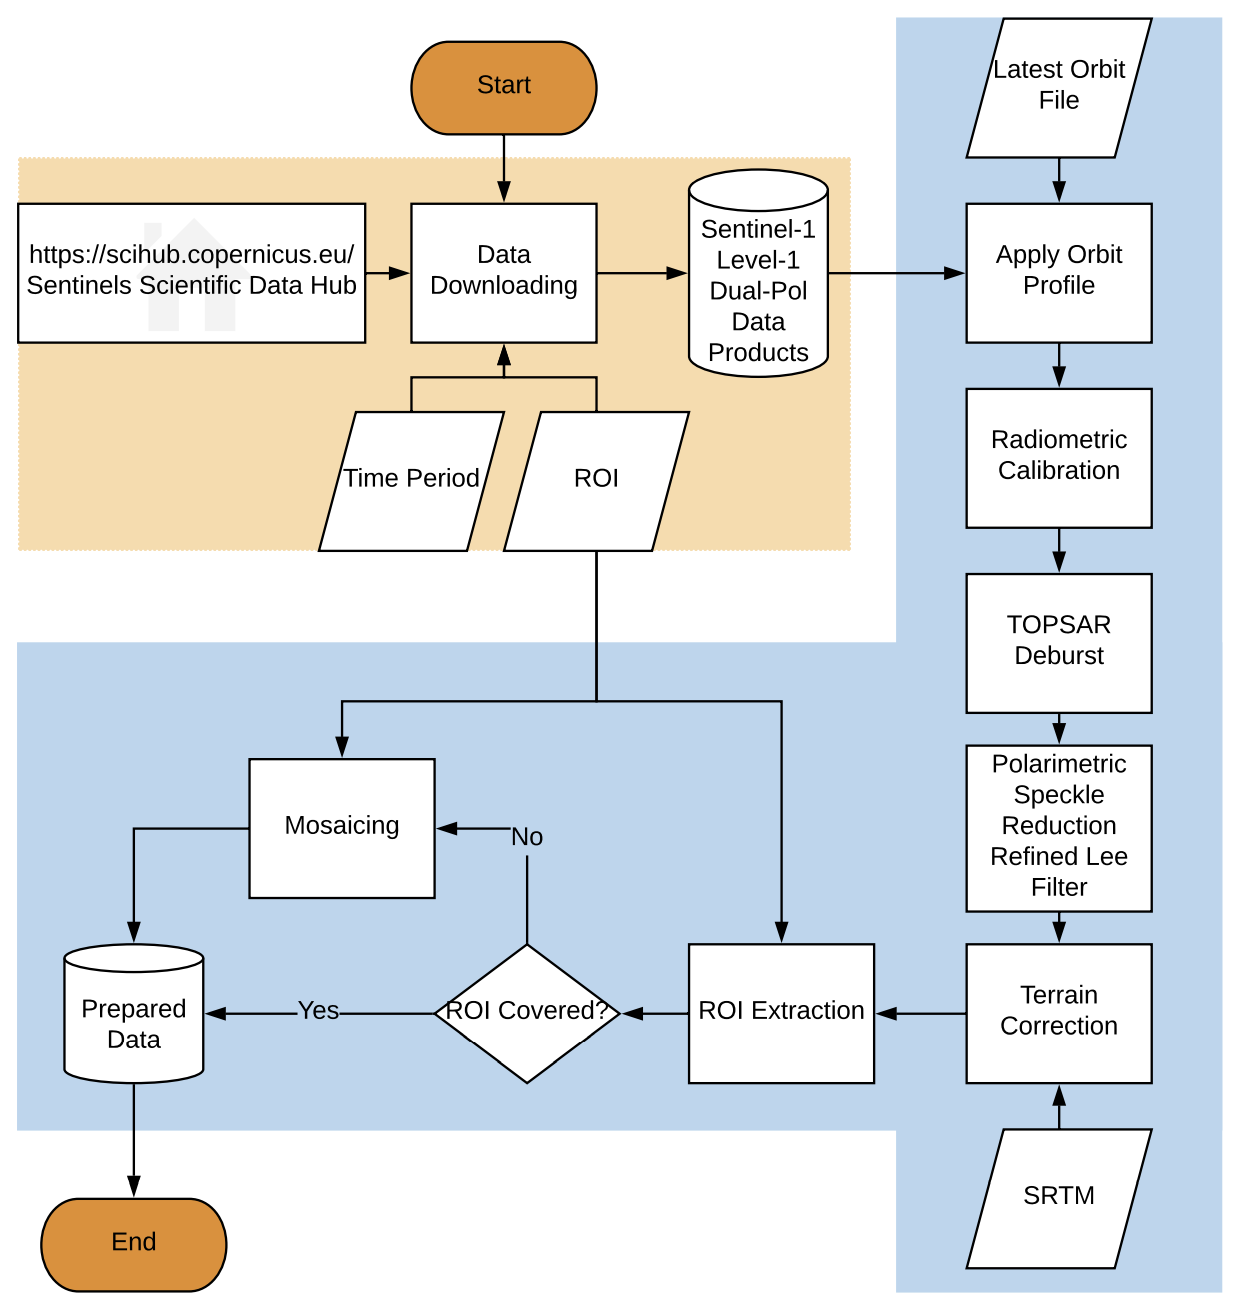
\includegraphics[scale=0.27]{Images/Hu_2018_Data_Preparation.PNG}}
		\caption{Sentinel-1 data processing flowchart, provided by \cite{Hu_2018}. The orange area is the data collection and the blue area is the data processing done in SNAP.}
		\label{img:Hu_2018_Data_Preparation}
	\end{figure}
	
	\subsection{Sentinel Application Platform}
	The Sentinel Application Platform (SNAP) is an open access graphical user interface created to process SAR data from various missions, including Sentinel.

	\paragraph{Calibration}
	Before the SAR data can be used it must first be calibrated. 
	Sentinel data comes with calibration files that are used by SNAP to correctly represent the radar backscatter of the reflecting surface.

	\paragraph{TOPSAR Deburst}
	The IW acquisition mode captures three swath's per polarization, resulting in six images for dual-pol data.
	The TOPSAR Deburst is used to merge the six images into one image.
	
	\paragraph{Speckle Reduction}
	SAR images come with speckle noise, generated by the interference of reflected waves \cite{Filipponi_2019}, which reduces the quality of the images.
	Speckle noise filters are used to reduce the noise, but a careful balance is needed, since removing speckle also results in loss of detailed information \cite{Yommy_2015}. 
	The refined Lee filter, available in SNAP, is a popular filter because of its superior performance in preserving edges, linear features, and texture information \cite{Filipponi_2019}.
	
	\paragraph{Terrain Correction}
	% YVETTE - need to add this section!!!
	
	
% ------------------------------------------------------------------------------------------------------------
% ~ ~ ~ ~ ~ ~ ~ ~ ~ ~ ~ ~ ~ ~ ~ ~ ~ ~ ~ ~ ~ ~ ~ ~ ~ ~ ~ ~ ~ ~ ~ ~ ~ ~ ~ ~ ~ ~ ~ ~ ~ ~ ~ ~ ~ ~ ~ ~ ~ ~ ~ ~ ~ ~ 
% ------------------------------------------------------------------------------------------------------------
	\begin{figure}[htbp]
		\centerline{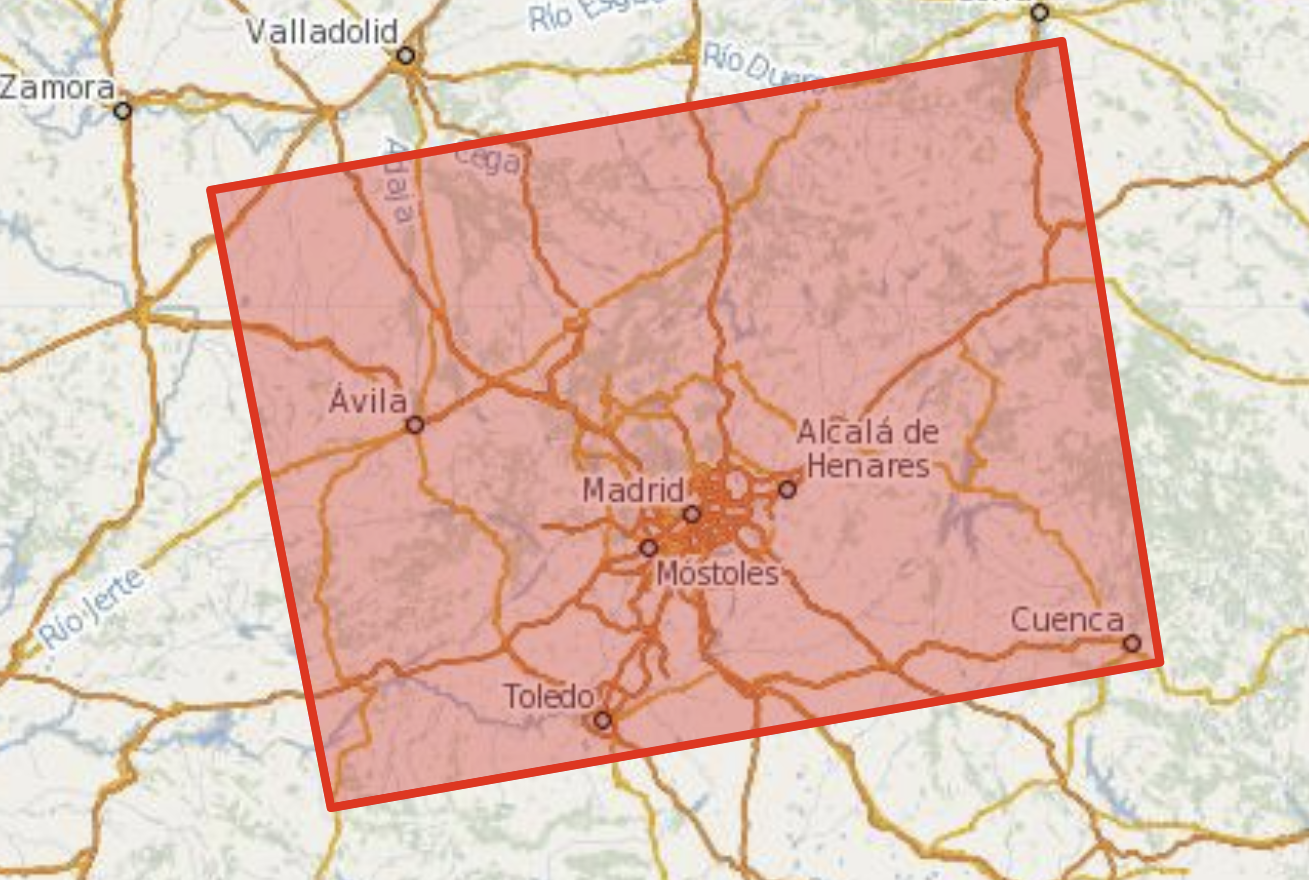
\includegraphics[scale=0.25]{Images/Madrid_SLC_IW_Data.PNG}}
		\caption{The region of interest from the Sentinel-1 data acquired on April 2, 2022.}
		\label{img:Madrid_SLC_IW_Data}
	\end{figure}

	\section{Results}
	The time period and region of interest were chosen arbitrarily. 
	The acquired data was from April 2, 2022 6:11 PM, which happened to capture Madrid, Spain. The region is shown in Figure \ref{img:Madrid_SLC_IW_Data}. 
	
	The 'Apply Orbit Profile' step of the data preprocessing was disregarded because orbit profiles are not available until 21 days after data acquisition.
	
	The radiometric calibration is currently failing due to a buffer overflow, that problem is currently being investigated.
	


% ------------------------------------------------------------------------------------------------------------
% ~ ~ ~ ~ ~ ~ ~ ~ ~ ~ ~ ~ ~ ~ ~ ~ ~ ~ ~ ~ ~ ~ ~ ~ ~ ~ ~ ~ ~ ~ ~ ~ ~ ~ ~ ~ ~ ~ ~ ~ ~ ~ ~ ~ ~ ~ ~ ~ ~ ~ ~ ~ ~ ~ 
% ------------------------------------------------------------------------------------------------------------
	\section{Conclusion}
	



% ------------------------------------------------------------------------------------------------------------
% ~ ~ ~ ~ ~ ~ ~ ~ ~ ~ ~ ~ ~ ~ ~ ~ ~ ~ ~ ~ ~ ~ ~ ~ ~ ~ ~ ~ ~ ~ ~ ~ ~ ~ ~ ~ ~ ~ ~ ~ ~ ~ ~ ~ ~ ~ ~ ~ ~ ~ ~ ~ ~ ~ 
% ------------------------------------------------------------------------------------------------------------
% USEFUL LINKS: 
% Worldview-3 dataset (mentioned in a few papers):
%	https://earth.esa.int/eogateway/catalog/worldview-3-full-archive-and-tasking
% GLCM textural metrics for remote sensing image analysis
%	https://rstudio-pubs-static.s3.amazonaws.com/536921_af2c31c083544a3a9588da9c86692636.html
% Copernicus Open Access Hub (where to get Sentinel-1 data)
%	https://scihub.copernicus.eu/userguide/
% Info on SAR bands
%	https://earthdata.nasa.gov/learn/backgrounders/what-is-sar
% SAR basics (using the SNAP program)
% 	http://step.esa.int/docs/tutorials/S1TBX%20SAR%20Basics%20Tutorial.pdf
% Sentinel-1 User Guides:
%	https://sentinels.copernicus.eu/web/sentinel/user-guides/sentinel-1-sar/naming-conventions
%	https://sentinel.esa.int/web/sentinel/technical-guides/sentinel-1-sar/products-algorithms/level-1-product-formatting
%	https://sentinels.copernicus.eu/web/sentinel/user-guides/sentinel-1-sar/acquisition-modes


	\nocite{*}
	\printbibliography
	
\end{document}
